% Licensed to the Apache Software Foundation (ASF) under one or more
% contributor license agreements. See the NOTICE file distributed with
% this work for additional information regarding copyright ownership.
% The ASF licenses this file to You under the Apache License, Version 2.0
% (the ``License''); you may not use this file except in compliance with
% the License. You may obtain a copy of the License at
%
% http://www.apache.org/licenses/LICENSE-2.0
%
% Unless required by applicable law or agreed to in writing, software
% distributed under the License is distributed on an ``AS IS'' BASIS,
% WITHOUT WARRANTIES OR CONDITIONS OF ANY KIND, either express or implied.
% See the License for the specific language governing permissions and
% limitations under the License.

\begin{changemargin}{1.5in}{0in}

\section{Overview}

The MetaCarta GTS appliance indexes documents and allows users to
search these documents based on both keywords and geographic
references. The MetaCarta JDBC Connector allows system administrators
to configure connections to SQL repositories and define jobs to
maintain synchronization between the repositories and the GTS
index. Currently, the JDBC Connector supports Oracle, Postgres SQL, MS
SQL Server (Version greater than 6.5), and Sybase (Version 10 and
greater) repositories.

This document specifies the means for connecting to these repositories,
indexing files from these repositories, and maintaining connections to
these repositories.

\subsection{Assumptions}

This document assumes you have a basic level of familiarity with GTS
appliance administration. This document also assumes that you have a
basic understanding of the repositories to which you are trying to
connect. If you need more information about the MetaCarta GTS
appliance, please read the \documentref{MetaCarta GTS Administrator's
Guide} stored on the appliance at
\dirpath{/usr/share/doc/metacarta/AdminGuide.pdf}. For more
information about your SQL database, please see your database
documentation or database administrator.

Throughout this document, we assume that your appliance is named \\
\url{metacarta.example.com}. 

\section{Installation}

The JDBC Connector is included with the Connector Addon
available from Metacarta. % Licensed to the Apache Software Foundation (ASF) under one or more
% contributor license agreements. See the NOTICE file distributed with
% this work for additional information regarding copyright ownership.
% The ASF licenses this file to You under the Apache License, Version 2.0
% (the ``License''); you may not use this file except in compliance with
% the License. You may obtain a copy of the License at
%
% http://www.apache.org/licenses/LICENSE-2.0
%
% Unless required by applicable law or agreed to in writing, software
% distributed under the License is distributed on an ``AS IS'' BASIS,
% WITHOUT WARRANTIES OR CONDITIONS OF ANY KIND, either express or implied.
% See the License for the specific language governing permissions and
% limitations under the License.

If you have not already installed the Connector Addon, you should use
the Connector Addon DVD to install it using the following steps:

\begin{enumerate}

\item Insert the DVD in your appliance.

\item Install the Connector Addon:

\begin{console}

metacarta:\~{}\$ sudo upgrade\_control install --from-dvd 

\end{console}

This will restart your appliance and eject the Connector Addon DVD.

\item Upgrade your license file, if necessary. For instructions,
see the \documentref{MetaCarta Appliance Administrator's Guide} or 
contact Customer Support (see page \pageref{SupportContact}).

\end{enumerate}

The Connector Addon cannot be uninstalled.

\subsection{Remote Updates}

In some cases, it may be very difficult to get physical access to an
appliance in order to install new software. To make the installation
process easier, MetaCarta provides a mechanism for remote
installations.  MetaCarta will provide you with ISO images of the
software you need upon request.  In brief, you can install the 
Connector Addon from ISO with the following command:

\begin{console}

metacarta:\~{}\$ sudo upgrade\_control install /path/to/iso.iso

\end{console}

For more information on the use of ISO
images for remote installations, see the \documentref{MetaCarta GTS
Administrator's Guide} stored on the appliance at
\dirpath{/usr/share/doc/metacarta/AdminGuide.pdf}.


\section{Configuration}

\subsection{Access to the Connector}

The administrator to the JDBC Connector % Licensed to the Apache Software Foundation (ASF) under one or more
% contributor license agreements. See the NOTICE file distributed with
% this work for additional information regarding copyright ownership.
% The ASF licenses this file to You under the Apache License, Version 2.0
% (the ``License''); you may not use this file except in compliance with
% the License. You may obtain a copy of the License at
%
% http://www.apache.org/licenses/LICENSE-2.0
%
% Unless required by applicable law or agreed to in writing, software
% distributed under the License is distributed on an ``AS IS'' BASIS,
% WITHOUT WARRANTIES OR CONDITIONS OF ANY KIND, either express or implied.
% See the License for the specific language governing permissions and
% limitations under the License.

must have
access to the web interface at
\url{http://metacarta.example.com/crawler/}. In the default appliance
security setup, you must have a Basic Authentication account
configured for access to the Connector web interface at
\url{http://metacarta.example.com/crawler/}.  If you are not an appliance
administrator, please ask the appliance administrator to give you such
an account.

An appliance administrator can create an account with access to the
ingestion interface (in this case, username {\tt fred} and password
{\tt ginger}) by running the following command on the appliance:

\begin{console}
metacarta:\~{}\$ basic\_auth\_control add ingest\_users fred:ginger 
\end{console}

Depending on how you have configured authentication using the
\command{auth\_control} tool, you may need to make changes other than
adding yourself to the ingest\_users group. For more information on
security configuration and \command{auth\_control}, see the Security
Administration section of the \documentref{MetaCarta Appliance
Administrator's Guide}.



\section{Collecting Documents From Repositories} % Retitle this, yo.

The Connector Framework manages retrieving documents from different
repositories through \emph{jobs}. Jobs can be scheduled to run
regularly; each job connects to a single repository using a particular
set of credentials. Each job is tied to a \emph{repository
connection}. Repository connections contain information allowing the
connector framework to connect to a given repository. A repository
connection may be tied to an \emph{authority connection}, which
manages document security. While using the JDBC Connector to connect
to a SQL database, no authority connection is needed; you can simply
create a repository connection.



\subsection{Creating Repository Connections}

In order to create jobs to ingest documents, you need to create a
repository connection. To do so, click ``List Repository
Connections'' on the sidebar menu. Then, when presented with the list
of repository connections, click ``Add a new connection.'' You will
see the following two tabs:

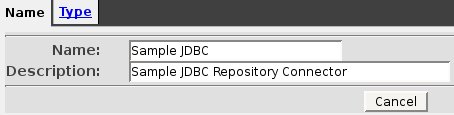
\includegraphics[width=300pt]{JDBC-edit-repository-tab1}

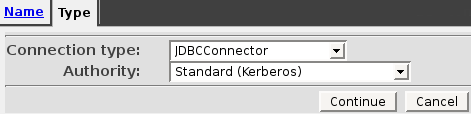
\includegraphics[width=300pt]{JDBC-edit-repository-tab2}

% Licensed to the Apache Software Foundation (ASF) under one or more
% contributor license agreements. See the NOTICE file distributed with
% this work for additional information regarding copyright ownership.
% The ASF licenses this file to You under the Apache License, Version 2.0
% (the ``License''); you may not use this file except in compliance with
% the License. You may obtain a copy of the License at
%
% http://www.apache.org/licenses/LICENSE-2.0
%
% Unless required by applicable law or agreed to in writing, software
% distributed under the License is distributed on an ``AS IS'' BASIS,
% WITHOUT WARRANTIES OR CONDITIONS OF ANY KIND, either express or implied.
% See the License for the specific language governing permissions and
% limitations under the License.

\begin{picture}(1,1)
  \put(-100,15){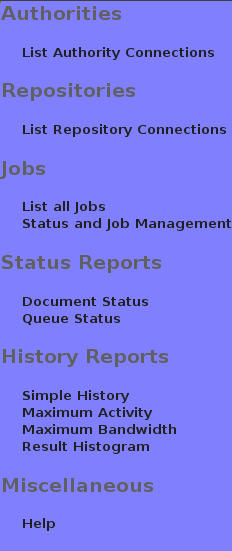
\includegraphics[width=80pt]{crawler-sidebar}}
\end{picture}


Now you must provide a name, description, and connector type for your
new repository connection. The name should be unique, as you will use
it to select this connection later when defining jobs. The description
should explain the repository connection to you or another
administrator.  The connector type is the type of repository from
which you will get documents, in this case a JDBCConnector. The
authority type is the type of authority from which you will get
authorization information. The JDBC Connector does not use an
administrator-created authority; you should simply select ``Standard
(Kerberos)'' here.

Once you have filled in those tabs, click Continue to be taken to the
repository-specific options.

% Licensed to the Apache Software Foundation (ASF) under one or more
% contributor license agreements. See the NOTICE file distributed with
% this work for additional information regarding copyright ownership.
% The ASF licenses this file to You under the Apache License, Version 2.0
% (the ``License''); you may not use this file except in compliance with
% the License. You may obtain a copy of the License at
%
% http://www.apache.org/licenses/LICENSE-2.0
%
% Unless required by applicable law or agreed to in writing, software
% distributed under the License is distributed on an ``AS IS'' BASIS,
% WITHOUT WARRANTIES OR CONDITIONS OF ANY KIND, either express or implied.
% See the License for the specific language governing permissions and
% limitations under the License.

\subsubsection{Configuring a JDBC Connector}

You must fill in the following tabs if you are configuring a JDBC
Connector:

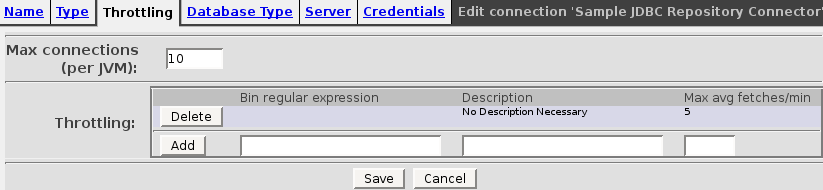
\includegraphics[width=300pt]{JDBC-edit-repository-tab3}

\begin{itemize}

\item \textbf{Max connections (per JVM):} Here you can set the maximum
number of connections to your repository.  \ifCombinedConnectorGuide
The maximum number of connections per JVM is important for three
reasons; licensing, appliance resources, and the possiblity of
overwhelming the ingestion interface. For a more complete explanation,
see the Max Connections item on page \pageref{maxrepocon}.\fi

\ifJDBCGuide
The maximum number of connections per JVM is important for three reasons.
First, the number of connections may impact the licensing on your document
server, depending on the repository.

Second, the number of connections may impact the resources
available on the appliance. If the connector framework is slowing down
your appliance, lowering this number should help.

Third, only ten document streams can be processed by the appliance
at one time.  If you are also using other repository connectors or
the \command{ingest} command on the appliance, you should reduce this
number to prevent contention for the Ingestion interface. The JDBC
Connector will never overwhelm the interface on its own, but when other
applications are also using the ingestion interface, it may be best to
set the number of repository connections to five or even fewer.
\fi


\item \textbf{Throttling:} Here you can set a maximum document fetch
rate for the repository connection.

The maximum fetch rate allows you to set three things: Expression,
description, and fetches per minute. Expression allows you to provide
a regular expression to match against document bins.  Each document
ingested through a connector is associated with one or more document
bins. These bins represent the servers that the connector interacts
with to obtain the document.  Typically, a document will be associated
with only one document bin, representing the repository server hosting
the document. For some repository connections, documents ingested
through the connector can be hosted by different servers. In the JDBC
Connector, documents only come from one server, which you will set on
the ``Server'' tab. Simply leave the expression blank; this will match
any server you enter on the ``Server'' tab.  All you need to set is
the number of document fetches per minute.  Description is an optional
field that allows you to provide a short text description of the
throttle.  Once you have set the fetch rate and optional description,
click Add.


\end{itemize}

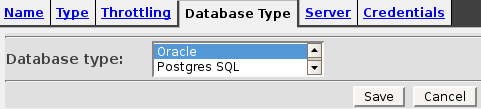
\includegraphics[width=300pt]{JDBC-edit-repository-tab4}

\begin{itemize}

\item \textbf{Database Type:} Here you should select the type of
database to which you are connecting. Currently supported databases
include Oracle, Postgres SQL, MS SQL Server (Version greater than
6.5), and Sybase (Version 10 and greater).

\end{itemize}

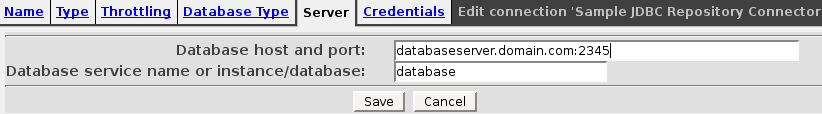
\includegraphics[width=300pt]{JDBC-edit-repository-tab5}

\begin{itemize}

\item \textbf{Server Database Host and Port:} Ask your database
administrator to provide you with the correct host name and port
number for your repository. This should be of the form
\url{databaseserver.domain.com:port}.

\item \textbf{Database service name or instance/database:} This should
be the name of the database you wish to crawl in the form
\command{database} or \linebreak \command{instance/database}.

\end{itemize}

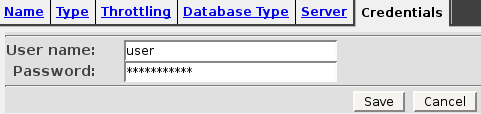
\includegraphics[width=300pt]{JDBC-edit-repository-tab6}

\begin{itemize}

\item \textbf{Name:} This is the username that the GTS appliance will
use to connect to your database server. It is recommended that the GTS
appliance be given its own username in the system. The appliance will
need to be granted appropriate permissions to select from the tables
you wish to crawl.

\item \textbf{Password:} This is the password that corresponds to the
username provided above.

\end{itemize}


After entering this information, you will be taken to the repository 
connection status page for this repository:

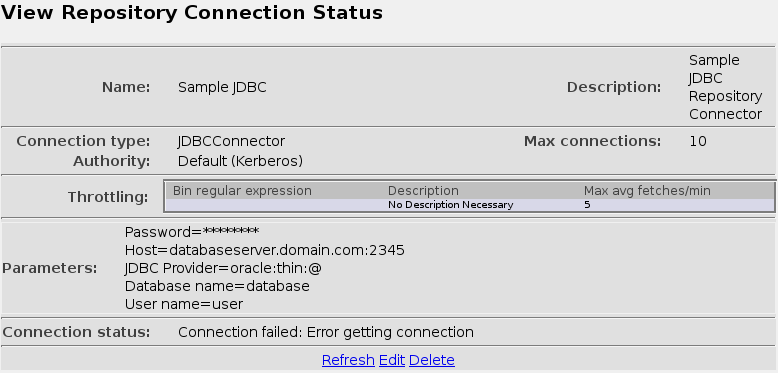
\includegraphics[width=300pt]{JDBC-view-repo-conn-status}

In this example (which does not contain accurate information for any
JDBC Connector), the Connection Status is ``Connection failed.''
If you see this message, you most likely have incorrectly entered one
of the fields, and should click ``Edit'' to fix the data. If you have
entered everything as you intended, please inform your database administrator;
you may not have been given the correct information.


\subsection{Creating and Running Jobs}

To run a job, click ``Status and Job Management'' on the sidebar menu.
You can run or edit existing jobs from this menu.

To create a new job, click ``List All Jobs'' on the sidebar menu. Then, when
presented with the list of current jobs, click ``Add a new job.'' You
will be presented with two tabs, in which you must fill in the following
information:

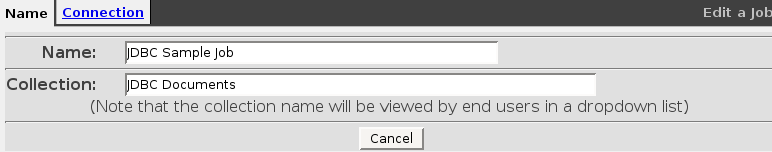
\includegraphics[width=300pt]{JDBC-edit-job-tab1}

\begin{itemize}

\item \textbf{Name:} The name of the job. You will use this to identify
the job later.

\item \textbf{Collection:} The collection name metadata for all
documents in this job. End users can use this name to select the set
of documents in this job. For more information on collection name
metadata, please see the \documentref{MetaCarta GTS Administrator's
Guide}.

\end{itemize}

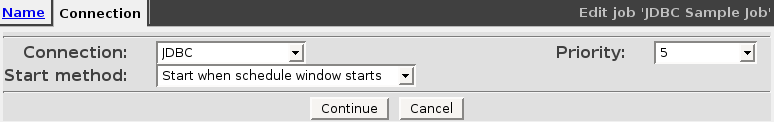
\includegraphics[width=300pt]{JDBC-edit-job-tab2}

\begin{itemize}

\item \textbf{Connection:} The name of the repository connection you
wish to use for this job. You select this from the list of repository
connections you have already made. You may have more than one job use
the same repository connection, but if you have two jobs crawl the same
documents, the documents will have the metadata and collection name
associated with whatever job crawled the document most recently. This
will cause unpredictable results when searching those collections,
searching for those documents, or trying to delete those collections.
We recommend never crawling the same document in two different jobs.

\item \textbf{Start method:} Whether you want to start this job the next
time jobs are scheduled to run (``Start when schedule window starts''),
immediately after you finish defining it (``Start even inside a schedule
window''), or not at all (``Don't automatically start this job'').

\item \textbf{Priority:} From 1 (highest) to 10 (lowest), the priority
this crawl should have if it must compete for resources with other
crawls on the appliance. You should not need to change this unless you
are running more than one crawl at the same time; if you are, assign a
higher priority to the crawls whose documents you want to be processed
preferentially before documents from other jobs.

\end{itemize}

After filling in those options, click ``Continue'' and you will be
presented with two additional repository-specific tabs.

% Licensed to the Apache Software Foundation (ASF) under one or more
% contributor license agreements. See the NOTICE file distributed with
% this work for additional information regarding copyright ownership.
% The ASF licenses this file to You under the Apache License, Version 2.0
% (the ``License''); you may not use this file except in compliance with
% the License. You may obtain a copy of the License at
%
% http://www.apache.org/licenses/LICENSE-2.0
%
% Unless required by applicable law or agreed to in writing, software
% distributed under the License is distributed on an ``AS IS'' BASIS,
% WITHOUT WARRANTIES OR CONDITIONS OF ANY KIND, either express or implied.
% See the License for the specific language governing permissions and
% limitations under the License.

\subsubsection{JDBC Job Options}

You must fill in the ``Scheduling,'' ``Queries,'' and ``Security''
tabs to configure a JDBC job.

\bigimage{JDBC-edit-job-tab3}

\ifJDBCGuide
% Licensed to the Apache Software Foundation (ASF) under one or more
% contributor license agreements. See the NOTICE file distributed with
% this work for additional information regarding copyright ownership.
% The ASF licenses this file to You under the Apache License, Version 2.0
% (the ``License''); you may not use this file except in compliance with
% the License. You may obtain a copy of the License at
%
% http://www.apache.org/licenses/LICENSE-2.0
%
% Unless required by applicable law or agreed to in writing, software
% distributed under the License is distributed on an ``AS IS'' BASIS,
% WITHOUT WARRANTIES OR CONDITIONS OF ANY KIND, either express or implied.
% See the License for the specific language governing permissions and
% limitations under the License.

\begin{itemize}
\label{scheduling}

\item \textbf{Schedule type:} Whether you want to scan every document
once or dynamically recrawl content in your repository. 

When scanning every document once, the crawler marks all documents that
have been previously crawled in this job as potentially to be deleted,
adds all seed documents to its queue and marks them as pending, processes
pending documents, marking them completed as they are ingested, and then
deleted all of the documents that were not recrawled. A document might
not be recrawled because it no longer exists, or the job specification
might have been changed to no longer include the document.

When dynamically recrawling documents, the crawler does not start by
marking all documents as potentially deletable; instead, it begins with
all of the seed documents, and continues adding to its list, periodically
re-adding the initial seed documents. If a document is removed from the
source, it will expire in the expiration interval (see below).

\item \textbf{Expiration Interval (if continuous):} The length of the
interval (in minutes) that the appliance will retain a document
crawled by this job after the document no longer appears in the
repository. After this interval, the missing document will be removed
from the appliance's index and archive. Leave the expiration interval
blank to keep missing documents indexed in GTS.

\item \textbf{Recrawl interval:} If you are dynamically recrawling
documents, how long, in minutes, the crawler should wait before
crawling documents a second time.

\item \textbf{Reseed interval:} If you are dynamically recrawling
documents, how long, in minutes, the crawler should wait before
looking for new documents to crawl. \ifMeridioGuide This connector
identifies all documents for ingestion through seeding; if the reseed
interval is infinite, the job will not ingest documents placed in the
repository during run time. (The job automatically reseeds whenever it
is started.) The default interval of 60 minutes is an appropriate
reseed rate. \fi \ifFilenetGuide This connector identifies documents
for ingestion during seeding. If you change the document inclusion
criteria, reseeding is required to identify new documents. Similarly,
documents placed in the repository while the job is running will not
be identified until the crawl is reseeded.  (The job automatically
reseeds whenever it is started.) The default interval of 60 minutes is
an appropriate reseed rate. \fi

\item \textbf{Scheduled time:} Allows you to define a time you wish
the job to run using a series of selection boxes. The first box refers
to the day of the week you wish the job to run, with an option to have
the job run any day of the week. The second box allows you to select
the start hour, with an option to start the job at any hour. The third
box allows you to specify which minute after the hour that you wish
the job to start. The fourth box allows you to specify what months of
the year you wish the job to run, with an option for the job to run
any month. The last box allows you to specify the day of the month you
wish the job to start, including any day of month.


You can scroll through each of the five boxes in this setting using
the arrow keys on your keyboard or by using the scroll bar on the
right side of the box.  If you want to select more than one value,
hold down control as you scroll and click the values that you want to
select. This allows you to define multiple windows with the same
length, for example by selecting Monday, Wednesday, and Friday at the
same time.

\item \textbf{Maximum run time:} The longest you will allow the job to
run, in minutes. For example, if you want to start a job at 2 AM but
force it to stop at 8 AM so that users have access to the repository,
you should set this value to 360 minutes. If the job is not complete by the
end time, documents that have already been found will be indexed, and
the rest of the crawl will continue at the beginning of the next
schedule interval. 

When you have defined the scheduled time and assigned a maximum run
time, click on the ``Add Scheduled Time'' button. A new schedule box
will appear below the scheduled time, allowing you to create
additional scheduled run times.

Here is a sample schedule for a job that will run every
Monday from 2 am to 6 am:

\begin{changemargin}{-.3in}{0in} 
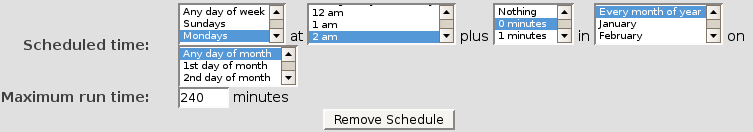
\includegraphics[width=300pt]{sample-schedule}
\end{changemargin}

If you do not have at least one scheduled time, the job will
only run when run manually (see page \pageref{ManageJobs}), and will
not automatically update the index on the appliance based on changes
to the repository.

You can remove a scheduled time by clicking the ``Remove Schedule''
button.

\end{itemize}

\fi

\ifCombinedConnectorGuide
This tab presents scheduling options. Here you can generate one or
more scheduled run times for the job. For a complete description of
the scheduling options, see the description starting on page
\pageref{scheduling}.
\fi

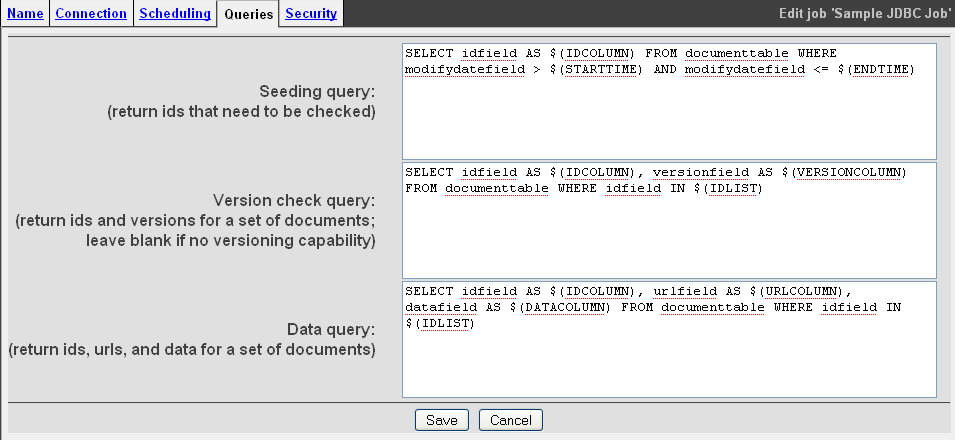
\includegraphics[width=300pt]{JDBC-edit-job-tab4}

In each of the three fields, you will need to construct an appropriate
SQL query. The sample queries shown include helper strings of the form
\command{\$(HELPER)} used by the connector, which are explained as they
appear.

\begin{itemize}

\item \textbf{Seeding Query:} The seeding query should return the
identifiers of documents in the repository that should be checked
against the files indexed in the GTS database. These identifiers
should be returned in a result-set as a column named
\command{\$(IDCOLUMN)}. The sample query shown above reads:

\begin{console}
SELECT idfield AS \$(IDCOLUMN) FROM documenttable WHERE modifydatefield
> \$(STARTTIME) AND modifydatefield <= \$(ENDTIME)

\end{console}

In this sample seeding query, identifiers from \command{idfield} for
entries from table \command{documenttable} are returned as a column
named \command{\$(IDCOLUMN)}. This example uses a \command{WHERE}
expression to limit the returned identifiers to entries with a
modified date, \command{modifydatefield}, in the range specified by
\command{\$(STARTTIME)} to \command{\$(ENDTIME)}. The time range spans
from the last time the job was run to the current start time, as
maintained by the GTS appliance. Time filtering is not a required part
of this query, but it helps reduce the number of documents being
passed to the ingestion interface by filtering out documents that have
not been modified since the last time the job was run.

A seeding query must be included. The seeding query must return a
column named \command{\$(IDCOLUMN)} as part of its result-set.

\note{Use caution when constructing queries that include time-based
components. \command{\$(STARTTIME)} and \command{\$(ENDTIME)} provide
times in milliseconds since epoch. If the modified date field is not
in this unit, the seeding query may not select the desired document
identifiers. You should convert \command{\$(STARTTIME)} and
\command{\$(ENDTIME)} to the appropriate timestamp unit for your system.

The following table gives several sample query fragments that can be
used to convert the helper strings \command{\$(STARTTIME)} and
\command{\$(ENDTIME)} into other date and time types. The first column names
the SQL database type that the following query phrase corresponds to,
the second column names the output data type for the query phrase, and
the third gives the query phrase itself using \command{\$(STARTTIME)}
as an example time in milliseconds since epoch. These query phrases
are intended as guidlines for creating an appropriate query phrase in
each language. Each query phrase is designed to work with the most
current version of the database software available at the time of
publishing for this document. If your modified date field is not of
the type given in the second column, the query phrase may not provide
an appropriate output for date comparisons.}

% Licensed to the Apache Software Foundation (ASF) under one or more
% contributor license agreements. See the NOTICE file distributed with
% this work for additional information regarding copyright ownership.
% The ASF licenses this file to You under the Apache License, Version 2.0
% (the ``License''); you may not use this file except in compliance with
% the License. You may obtain a copy of the License at
%
% http://www.apache.org/licenses/LICENSE-2.0
%
% Unless required by applicable law or agreed to in writing, software
% distributed under the License is distributed on an ``AS IS'' BASIS,
% WITHOUT WARRANTIES OR CONDITIONS OF ANY KIND, either express or implied.
% See the License for the specific language governing permissions and
% limitations under the License.

%BEGIN LATEX
\ifBigMargins\begin{changemargin}{-1.5in}{0in}\fi
\ifLittleMargins\begin{changemargin}{-.75in}{0in}\fi
%END LATEX

\begin{tabular}{|p{1in}|p{1in}|p{3.5in}|}

\hline

\textbf{Database Type}&\textbf{Date Type}&\textbf{Sample Query Phrase}\\

\hline

Oracle & \textit{date} & \command{ TO\_DATE ( '1970/01/01:00:00:00',
'yyyy/mm/dd:hh:mi:ss') + ROUND (\$(STARTTIME)/86400000)}\\

%Oracle & \textit{date} & \command{ TO_DATE ( '1970/01/01:00:00:00', 'yyyy/mm/dd:hh:mi:ss') + ROUND (\$(STARTTIME)/86400000)}\\

\hline

Oracle & \textit{timestamp} & \command{TO\_TIMESTAMP('1970-01-01 00:00:00')
+ interval '\$(STARTTIME)/1000' second}\\

\hline

Postgres SQL & \textit{timestamp} & \command{date '1970-01-01' + interval
'\$(STARTTIME) milliseconds'}\\

\hline

MS SQL Server ($>$6.5) & \textit{datetime} & \command{DATEADD(ms,
\$(STARTTIME), '19700101') }\\

\hline

Sybase (10+) &  \textit{datetime} &\command{DATEADD(ms,
\$(STARTTIME), '19700101') }\\

\hline

\end{tabular}
%BEGIN LATEX
\ifBigMargins\end{changemargin}\fi
\ifLittleMargins\end{changemargin}\fi
%END LATEX


\item \textbf{Version Check Query:} If your document system has
versioning capabilities, a version check query should be used to
filter documents based on version. The sample version query shown
above reads:

\begin{console}
SELECT idfield AS \$(IDCOLUMN), versionfield AS \$(VERSIONCOLUMN) FROM
documenttable WHERE idfield IN \$(IDLIST)
\end{console}

The sample query returns a column
named \command{\$(IDCOLUMN)} of identifiers from \command{idfield} and a
column named \command{\$(VERSIONCOLUMN)} of version numbers from
\command{versionfield} from entries in the table \command{documenttable}
whose identifiers were passed to this query by the job process using
the input \command{\$(IDLIST)}.

A version check query is not required. If your document system does
not have versioning capability, leave this query blank.

\item \textbf{Data Query:} A data query returns the identifiers, URLs,
and data for a document. The sample data query shown above reads:

\begin{console}
SELECT idfield AS \$(IDCOLUMN), urlfield AS \$(URLCOLUMN), datafield AS
\$(DATACOLUMN) FROM documenttable WHERE idfield IN \$(IDLIST)
\end{console}

This sample data query returns three columns, a column named\linebreak
\command{\$(IDCOLUMN)} of identifiers from \command{idfield}, a column
named \command{\$(URLCOLUMN)} of document URLs from \command{urlfield},
and a column named \command{\$(DATACOLUMN)} of document contents from
\command{datafield}. These outputs are generated from entries in the table
\command{documenttable} whose identifiers were passed to this query by
the job process using the input \command{\$(IDLIST)}.

The data query is required. This query passes the documents and
associated information to the ingestion interface for either initial
ingestion or re-ingestion.

\end{itemize}

When possible, filter the files passed to the ingestion interface by
way of version, modification time, or other methods to reduce the
number of files that are re-ingested unnecessarily. This can
significantly improve the performance of the ingestion.

The exact entry form of helper strings varies depending on the type of
database being used. In the case of Postgres SQL, MS SQL Server, and
Sybase, the helper strings should just be entered as shown in the
sample queries, as \command{\$(HELPER)}. In the case of Oracle, the
helper strings naming columns should be enclosed in double
quotation marks, as \command{\char34\$(IDCOLUMN)\char34},
\command{\char34\$(VERSIONCOLUMN)\char34},\linebreak
\command{\char34\$(URLCOLUMN)\char34}, and
\command{\char34\$(DATACOLUMN)\char34}, while the helper strings
\command{\$(IDLIST)}, \command{\$(STARTTIME)}, and
\command{\$(ENDTIME)} should be left as shown.

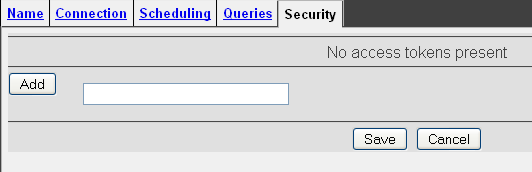
\includegraphics[width=300pt]{JDBC-edit-job-tab5}

If you wish to enable security, the user permissions you enter here will
be ingested with each document in this job. Otherwise, all documents in
this job will be ingested without permissions.

\item \textbf{Access Tokens:} To specify your own ACLs for files ingested
through this job, you can specify enter one or more ACL identifiers into
this field and click the ``Add'' button. The ACL identifiers will appear
in a list. You can continue to add more ACL identifiers using the ``Add''
button, or remove them using the ``Delete'' button that appears next to
each ACL identifier.

After entering this information, you will be taken to the status page
for this job:

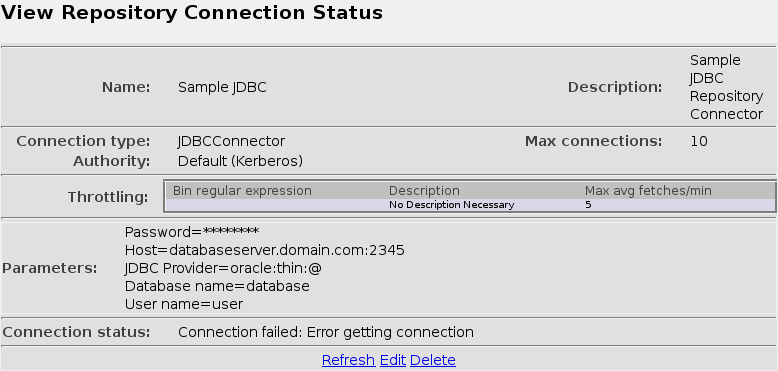
\includegraphics[width=300pt]{JDBC-view-job-status}


\subsection{\label{ManageJobs}Status and Job Management}

You can then look at the status of your job by clicking ``Status and 
Job Management'' on the sidebar. You will see a list of one or more jobs
much like this one:

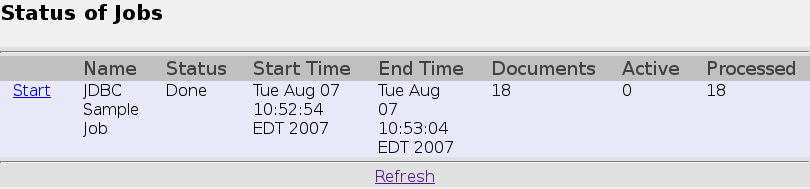
\includegraphics[width=300pt]{JDBC-jobs-list}

You can start any crawl you like immediately from this interface by
clicking ``Start'' next to the name of the crawl. This interface also
allows you to see how many documents have been crawled; this information
may help you structure and plan future crawls.

\note{Refresh this page by clicking the ``Refresh'' link at the bottom
of the page, not by clicking your browser's reload button.}

\section{Reports}

The Connector interface can generate four types of reports:

\begin{itemize}

\item Simple History, which lets you list an ordered set of log events
based on chosen criteria

\item Maximum Activity, which lets you see the period of time in
which a certain event happened most often

\item Maximum Bandwith, which lets you see the period of time in
which the most bandwidth was used 

\item Result Histogram, which provides log information that would be
appropriate for constructing a histogram or other diagram

\end{itemize}

Each of these reports allows you to specify a connection, one or more
activities, a start time, an end time, an entity match, and a result code
match.  Some also allow you to specify an identifier class description
and a sliding window size. This section will show sample results for
each type of report and an explanation of the fields selected.

\subsection{Simple History}

This report was generated by selecting ``JDBC Connection to Database,'' 
clicking Continue, selecting ``document ingest,'' and clicking Go.

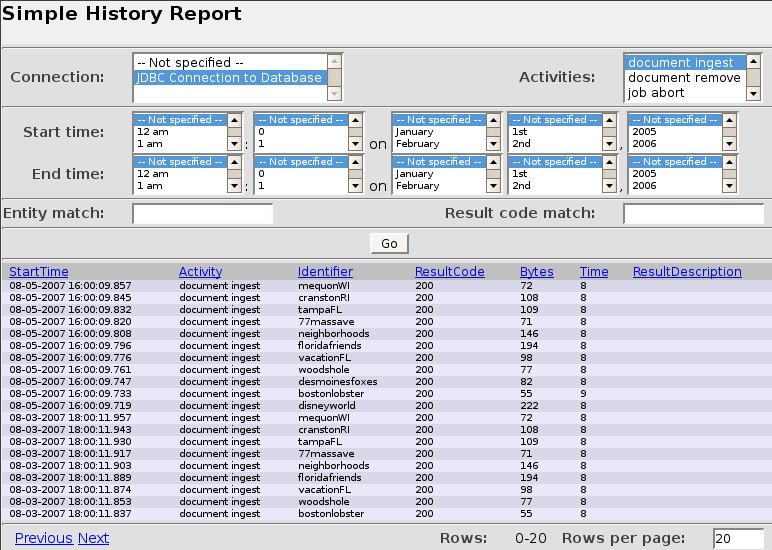
\includegraphics[width=300pt]{JDBC-simple-history-report}

\begin{itemize}

\item \textbf{Connection:} The repository connection from which to generate
a report.

\item \textbf{Activities}: What crawler activities you would like to see. 
Your options are document ingest, document remove, fetch document, find 
documents, job abort, job continue, job end, job start, and job wait. 

\item \textbf{Start time}: The earliest time in the crawler logs to be
considered for this query.  Choose ``Not specified'' for any field to
start at the beginning of the crawler's logs.

\item \textbf{End time:} The latest time in the crawler logs to be
considered for this query. Choose ``Not specified'' for any field 
to end at the current time.

\item \textbf{Entity match:} A regular expression to limit the
Identifier field. If the entity match field in the example above had
been \texttt{\^{}17}, only document fetches with Identifiers starting
with 17 would be shown.

\item \textbf{Result code match:} A regular expression to limit the
ResultCode field.

\end{itemize}

You can sort the history report by any of the returned fields; to do so,
click the field names.

\note{If you are not familiar with regular expressions,
there are a variety of tutorials available on the web,
including \url{http://gnosis.cx/publish/}\linebreak
\url{programming/regular_expressions.html} and
\url{http://perldoc.}\linebreak\url{perl.org/perlrequick.html}. If you
still have difficulty with these settings, please contact Customer Support
(see page \pageref{SupportContact}).}

\subsection{Maximum Activity}

This report was generated by selecting ``JDBC Connection to Database,''
clicking Continue, selecting ``document ingest,'' changing the Identifier
class description, and clicking Go.

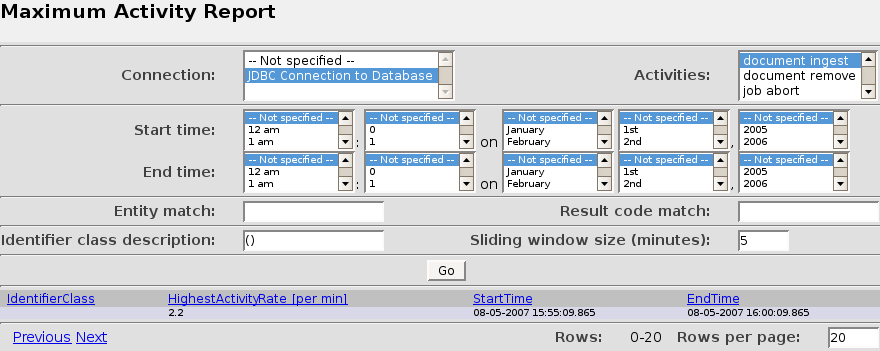
\includegraphics[width=300pt]{JDBC-maximum-activity-report}

This form offers two more fields than the previous form:

\begin{itemize}

\item \textbf{Identifier class description:} A regular expression
that determines how to group identifiers together. If this were set to
\texttt{(.*)}, there would be no grouping, and so there would be only one
ingestion event per document. If this were set to \texttt{(17)},
then all documents with identifiers beginning with 17 would be grouped
together. The setting in the example, \texttt{()}, groups all
documents together. Some other possibilities:

\begin{itemize}

\item \texttt{1(.)}: (up to) Ten groups of documents whose identifier starts
with 1, labeled 0-9, grouped by the second digit of their identifier.

\item \texttt{()}: One group of documents containing all documents 
regardless of identifier.

\item \texttt{17}: One group of documents whose identifier contains
the string ``17.''

\item \texttt{\^{}17}: One group of documents whose identifier \emph{starts}
with the string ``17.''

\end{itemize}

\item \textbf{Sliding window size}: The search interval in minutes.

\end{itemize}

The report returned will have only one result per group with one or more
documents in it, if there is a clear highest activity rate, or a list of
all the results tied for highest activity rate if there are more than one.

\subsection{Maximum Bandwidth}

This report was generated by selecting ``JDBC Connection to Database,''
clicking Continue, selecting ``document ingest,'' changing the Identifier
class description, and clicking Go.

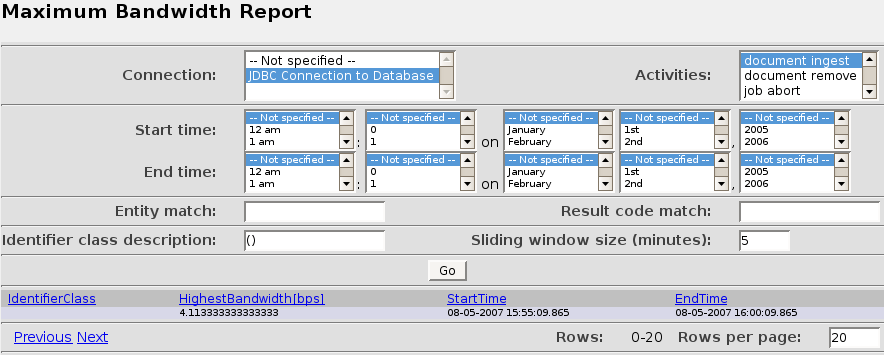
\includegraphics[width=300pt]{JDBC-maximum-bandwidth-report}

This form offers the same fields as the maximum activity form, and
returns similar results; instead of tracking events per time window,
it tracks the window with the highest average bandwith usage, measured
in bytes per second. Again, the identifier class description has been
changed to a regular expression that will match all identifiers (and
thus in this case documents).

\subsection{Result Histogram}

This report was generated by selecting ``JDBC Connection to Database,''
clicking Continue, selecting ``document ingest,'' and clicking Go.

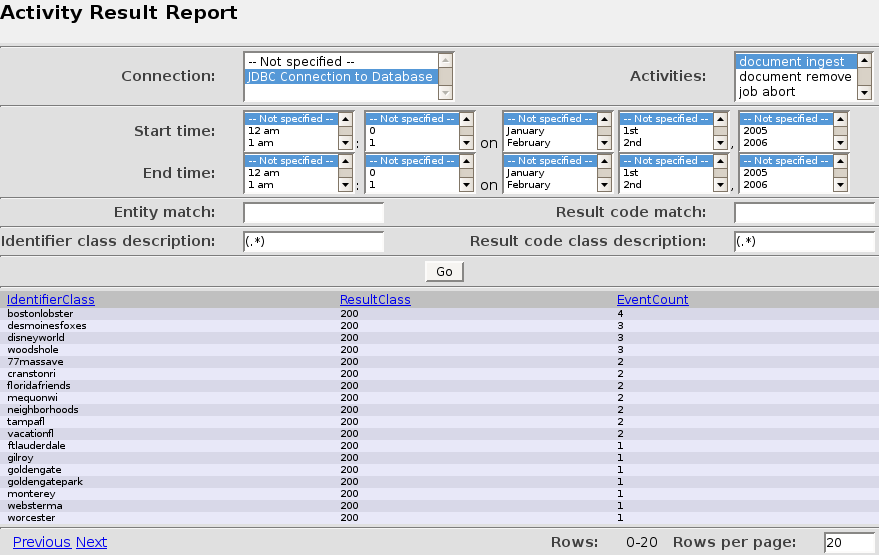
\includegraphics[width=300pt]{JDBC-activity-result-report}

This form adds one new field:

\begin{itemize}

\item \textbf{Result code class description:} A regular expression that
determines how to group result classes together; like Identifier class
descriptions but for result classes.

\end{itemize}

This report does not produce an actual histogram, but provides data that
could be used to generate histograms.  

% This is a little sparse, but that's basically all this is, so.

\end{changemargin}
